30. $\cfrac{(x^2-4x+4)(9-x^2)}{x^2+8x+16}\leqslant0\Leftrightarrow\cfrac{-(x-2)^2(x-3)(x+3)}{(x+4)^2}\leqslant0.$ Применив метод интервалов, найдём ответ: $x\in
(-\infty;-4)\cup(-4;-3]\cup\{2\}\cup[3;+\infty).$
\begin{figure}[ht!]
\center{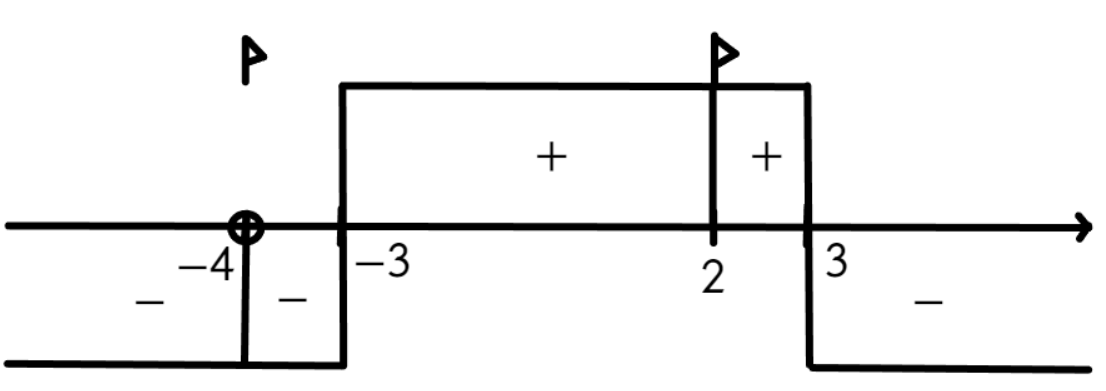
\includegraphics[scale=0.35]{ner9-30.png}}
\end{figure}\\
